% Diagrama de lo que espera hacer mi algorimto con una caja negra que es un sistema automl. Esperar que el sistema se actualize solo!!!!!
% Escribir que es lo que espera mi algoritmo caja negra, y que es lo que retorna !!!!
% Escribir como si todo fuera desde yo, usando el imperseanl (No la primera persona)

\chapter{AutoML Heter\'ogeneo Multiobjetivo}\label{chapter:proposal}

% Aqui poner flujo
% Seguido por parrafo que describe dicho flujo

\begin{figure}[ht]
    \centering
    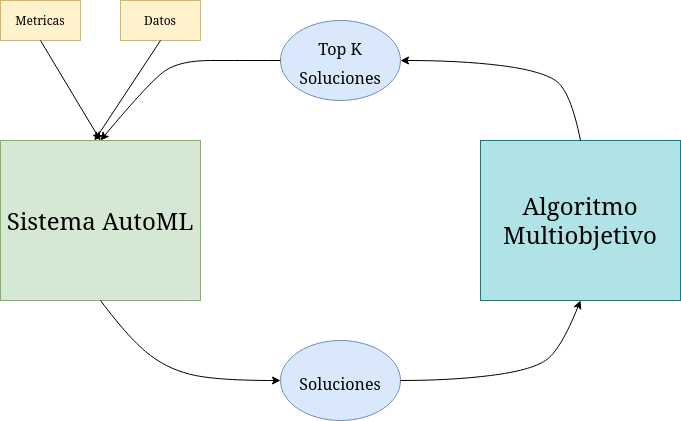
\includegraphics[scale=0.60]{Pictures/automl_moo_proposal.png}
    \caption{Flujo general de la propuesta}\label{proposal:fig:flux}
\end{figure}

Se propone como soluci\'on al  \textit{problema multiobjetivo en AutoML} (\ref{proposal:moo-automl-problem}) un algoritmo que utiliza como caja negra un sistema AutoML que sea capaz de producir una poblaci\'on inicial aleatoria de flujos. El algoritmo selecciona los mejores flujos utilizando un metodo de ordenaci\'on multiobjetivo y pide al sistema AutoML que genere y evalue una poblaci\'on a partir de los flujos escogidos como los m\'as aptos. 
%Se espera que este, partiendo de los mejores flujos sea capaz de producir una nueva generaci\'on manteniendo estos rasgos. 
Se repite este paso hasta que se cumpla el criterio de parada, en donde se devuelven las mejores respuestas encontradas hasta el momento con respecto a todas las iteraciones.


% Despues se define mas formalmente
\begin{definition}
El sistema toma como entrada un sistema de Aprendizaje de M\'aquina Automatizado $\mathcal{A}$ tal que $\mathcal{A}(D, M, P) = TP$ donde $D = \{(x_1, y_1), (x_2, y_2), ..., (x_n, y_n)\}$ representa un conjunto de datos de entrada, $M = \{f_1, f_2, ..., f_m\}$ un conjunto de m\'etricas a evaluar y $P = \{p_1, p_2, ..., p_k\}$ una serie de modelos de Aprendizaje Autom\'atico por los cuales se gu\'ia $\mathcal{A}$ para producir una nueva poblaci\'on de flujos $TP$. El objetivo del sistema es producir una conjutno de flujos de Aprendizaje Autom\'atico $P$ que sean una muestra representativa del frente de Pareto utilizando un algoritmo evolutivo multiobjetivo  $\mathcal{H}$ tal que $\mathcal{H}(TP) = P$ en cierto n\'umero de iteraciones determinado por un criterio de parada. 
\end{definition}

\begin{algorithm}[H]\caption{Flujo del Sistema}
    \KwIn{$\mathcal{A}$, D, M}
    \KwOut{P}
    
    $TP \gets \mathcal{A}(D, M, \emptyset)$ \tcp*{Se obtiene poblaci\'on inicial aleatoria}
    \While{no se cumplan condiciones de parada}{
        $P = \mathcal{H}(TP)$ \tcp*{Se extraen los m\'as aptos de una poblaci\'on} 
        $TP = \mathcal{A}(D, M, P)$ \tcp*{Se genera una nueva poblaci\'on}
    }
\end{algorithm}

% Despues aqui hablo sobre como se puede crear una separacion entre sistema AutoML y Algoritmo de Ordenacion
Las soluciones del problema pertencen al espacio de decisi\'on $\mathcal{X}$. La evaluaci\'on de estos pertencen a $\mathcal{Y}$ donde $\mathcal{Y} \subseteq \mathbb{R}^m$, donde $m$ es la cantidad de m\'etricas a evaluar. El sistema de AutoML trabaja sobre $\mathcal{X}$ y hace un relaci\'on uno a uno en $\mathcal{Y}$ al evaluarlas. Luego en $\mathcal{Y}$ se escogen los mejores valores de acuerdo al algoritmo multiobjetivo escogido. Estas mejores soluciones se le pasan al sistema AutoML. Por tanto es posible separar adecuadamente a esto entes.

% Como ambos trabajan en espacios distintos entonces se puede crear esta separacion que permite que optimizar simultanemanete utilizando a AutoGOAL como caja negra
% Al fin y al cabo se puede ver que se usa el sistema AutoML como un mapping entre dos espacios. Del espacio de  soluciones a sus evaluaciones.

El sistema AutoML necesario para esta propuesta se utiliza como caja negra y  es indiferente el tipo de soluciones que este produce, pueden ser redes neuroanles o flujos de Aprendiazaje Autom\'atico, basta con que sea capaz de producirlas y evaluarlas respecto a las diferentes m\'etricas de entrada.
Tambi\'en debe ser capaz de entender las carectr\'isticas que componen las soluciones m\'as aptas tal que en las subsecuentes iteraciones estas se conserven. Lograr esto \'ultimo requiere que el sistema tenga en cierta medida una implementaci\'on de algoritmos gen\'eticos para construir sus soluciones, por ende, la propuesta se adapta mejor a sistemas AutoML que utilizen programaci\'on evolutiva.

\section{Algoritmo de Optimizaci\'on Multiobjetivo}

El algoritmo trabaja con vectores debido a que optimiza para varias metricas, y no con un escalar que es trivial organizar. Como se meciona en \ref{background:def:moo} se hablar ahora de dominaci\'on y el adecuado ordenamiento es vital para escoger puntos del espacio que: (i) pertenzcan a los mejores frentes, (ii) que sean los elementos representativos del frente. Con este objetivo en mente se utiliza NSGA-II (\cite{deb2002fast}) como mecanismo a utilizar. Un algoritmo popular en el campo de la optimizaci\'on multiobjetivo, estar ampliamente probado y tener un buen rendimiento general. 

\begin{figure}[ht]\caption{Funcionamineto de NSGA-II}\label{proposal:fig:nsga2}
    \centering
    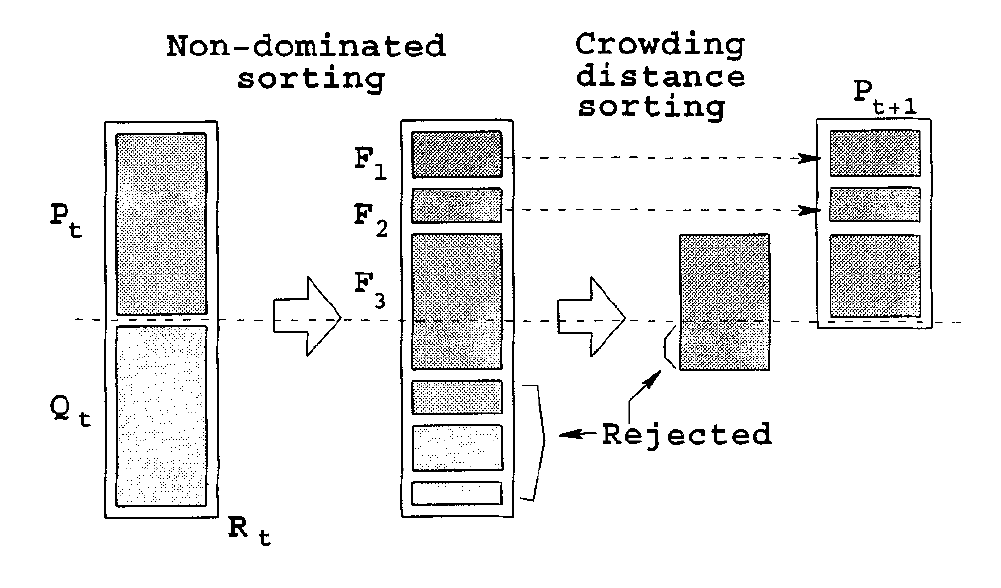
\includegraphics[scale=0.5]{Pictures/nsga2.png}
\end{figure}

El funcionamiento general de NSGA-II (ver figura \ref{proposal:fig:nsga2}) divide el proceso de ordenaci\'on en dos etapas.

Una primera etapa llamada \textit{Non Dominated Sort} donde se agrupan las soluciones de acuerdo a su \'indice de dominaci\'on. El \'indice de dominaci\'on de una soluci\'on est\'a determinado por la cantidad de diferentes soluciones que la dominan.
\begin{definition}
    \label{proposal:def:domination_index}
    Dado un vector $x$ y un conjunto $Y$ de vectores en el espacio objetivo $\mathcal{Y}$ tal que los vectores en $Y$ dominan a $x$ (i.e. $Y = \{y | y \succ x\}$) se dice que $Ind(x) = |Y|$.
\end{definition}
% (Explicar como es el non dominated sort, es el naive o el bueno)
El resultado de esta primera etapa es una lista de elementos $P = \{P^0, ..., P^k\}$ donde cada elemento $P^i = \{x | Ind(x) = i\}$ representa un conjutno de vectores con rango de dominaci\'on $i$. $P^0$ contiene las mejores vectores a los cuales nadie domina e idealmente ser\'ia una aproximaci\'on al frente de Pareto.

Es importante entender para la correctitud del aloritmo  que las soluciones que conforman un frente de rango $i$ no se \textit{Pareto dominan} ($\prec$) entre si.
%Es f\'acilmente demostrable que la \texit{Pareto dominacion (i.e. $\prec$)} cumple con la propiedad de transitividad (i.e. si $x \prec y$, $y \prec z$, entonces $x \prec z$) 
\begin{theorem}
Dado $P^i$, frente de rango $i$, resultado de efectuar obtenido por Non Dominated Sort sobre una conjutno soluci\'on entonces $\neg \exists x, y \in P^i$ tal que $x \prec y$
\end{theorem}
% Definir correctamente la prueba
Dado un frente de rango $i$ $F_i$, tal que existen soluciones $x, y \in F_i$ se asume que $x \prec y$. Como el \'inidice de dominaci\'on de $x$ es $i$ y $x \prec y$ y ($\prec$) es una operador transitivo entonces todos los que dominan a $x$ dominan a $y$, adem\'as del propio $x$, por tanto el inidice de dominaci\'on de $y$ ser\'ia $i+1$ lo que es una contradicci\'on porque $y \in F_i$. 

En la segunda etapa que los autores llaman \textit{crowding distance} (CD) se ordenan todos los conjuntos de $P$ con el objetivo de que los primeros elementos de estos sean lo m\'as representativo de dicho conjunto. La importancia de esta ordenaci\'on radica en el segundo paso, donde se escogen $k$ elementos mejores, y es necesario en muchas ocasiones que los primeros $p$ frentes no quepan completos. Entonces hay que picar un frente y se prefiere que se cojan los m\'as representativos de este.

%En la segunda etapa los vectores de cada frente obtenido se organizan utilizando \textit{crowding distance} (CD), uno de las contribuciones claves de NSGA-II (\cite{deb2002fast}). El prop\'osito de \textit{crowding distance} es estimar la densidad de las soluciones con respecto sus soluciones vecinas de tal manera que los primeros lugares pertenezcan a los elementos m\'as representativos de dicho frente.

% Imagen de crowding distance
Calcular el CD de cada soluci\'on require ordenarlas seg\'un su valor normalizado por cada funci\'on objetivo y calcular el promedio de la distancia entre una soluci\'on y sus dos adyacentes respecto a dicha funci\'on objetivo. Esta distancia resulta siendo el per\'imetro del cuboide formado usando los vecinos m\'as cercanos como v\'ertices. Los puntos que representan el m\'inimo y m\'aximo de al menos alguna funci\'on objetivo se les asigna \textit{crowiding distance} infinita. En \ref{proposal:alg:cd} se puede ver una representaci\'on del pseudoc\'odigo de esta ordenaci\'on.

\begin{algorithm*}[ht]
    \caption{Crowding Distance Sorting}
    \label{proposal:alg:cd}

    \tcp{F como entrada representa un frente de rango i}
    \KwIn{F} 
    \tcp{SF como salida representa el frente ordenado seg\'un CD}
    \KwOut{SF}
    \For{i desde 0 hasta $|F|$}{
        $F[i].dist \gets 0$ \;
    } 

    \ForEach{funcion objetivo $m$}{
        $F \gets ordenar(F, m)$ \tcp*{se ordena F con respecto a m}
        $F[0].dist \gets \infty$\;
        $F[|F|].dist \gets \infty$\;

        \For{i desde 2 hasta $|F| - 1$} {
            \begin{math}
                F[i].distance  = \frac{F[i].distance + (F[i + 1].m - F[i - 1].m)}{f^{max}_{m} - f^{min}_m}
            \end{math}
        }
    }
    $SF \gets ordenar(F, dist)$ \tcp*{se ordena F respecto a CD}
\end{algorithm*}


%tiene una adaptacion dependiendo de los datos de entrada, donde se recorren todos los posibles caminos de la gram\'atica y se quitan todas las producciones que no tienen sentido segun el conjunto de datos inicial (e.g. si la entrada son numeros no hay porque aplicar un algoritmo de lematizaci\'on).

% Se obtiene como resultado un Grafo Aciclico Dirigido (DAG), donde cada arista representa una la expansi\'on de alg\'un no terminal de la gram\'atica. Un camino recorrido por dicho DAG es una posible soluci\'on de autogoal, referido como flujo o \textit{pipeline} de Aprendizaje Autom\'atico. A las aristas del DAG mantienen las probabilidades contenidas en $Prob$. Para recorrer cada camino se lanza utiliza una variable aleatoria uniforme y seg\'un su valor se escoge una producci\'on. Esto se realiza hasta obtener nuevas soluciones, hasta obtener una gran poblaci\'on.


% % Al inicio en el DAG las probabilidades est\'an igualmente distribuidas segu\'un el nodo y la cantidad de aristas (1 nodo con 3 aristas, 0.33 para cada uno) sobre todas las producciones por cada regla de la gram\'atica y se actualizan al aplicar PGE con el individuo m\'as apto donde se alterna entre aumentar ligeramente la probabilidad de las producciones que utilizadas por este y disminuir la probabilidades de los que no fueron utilizadas. Alternar entre estas dos v\'ias evita la utilizaci\'on del mismo individuo en iteraciones consecutivas balanceando la exploraci\'on global con explotaci\'on local.

% Como se trata de un problema multiobjetivo y no existe el individuo m\'as apto, sino un conjunto de estos las probabilidas se adaptan secuencialmente teniendo en cuenta cada uno de estos individuos.

 % (\textit{Probabilistic Grammatic Evolution}).
% En PGE se propone un cambio de como se interpreta el genotipo, ya no es una lista de enteros, sino u
% Utiliza Algirmtos de Estimacion de Distribucion (\textit{Estimation of Distribution Algorithms, EDA}) una t\'ecninca probabi\'istica que remplaza los operadores de mutaci\'on y cruce por un sampleando sobre la probabiliad de distribuci\'on de las producciones obtenidas por mejor individuo, para luego generar una nueva poblaci\'on por cada cada generaci\'on. Las probabilidades comienzan todas inicializadas en igual proporci\'on  y se actualizan basado en la frecuencia de las reglas de produccion escogidas para obtener el individuo con el mayor rendimiento.
% Probablisitic Grammatical Evolution (PGE)  se apoya en una Gramatica Probabilistica Libre del Contexto (\textit{Probilistic Context-Free Grammatic Evolution} PCFGE) para realizar los mapeos de los fenotipos a los genotipos. PCFGE se establece como una tupla $PG = (NT, T, S, P, Prob)$ donde $Prob$  es un conjunto de probabilidades asocaido con cada regla de la gram\'atica. El genotipo en PGE es un vector de numeros fraccionarios, donde cada uno corresponer con la probabiliad de seleccion cierta regla de derivaci\'on.
% insetar ejemplo de PGE.
% En PGE las probabilidades se actualizan despues de cada generaci\'on  despues de evaluar la poblaci\'on generada, basasdo en cuantas veces cada regla de derivacion fue seleccionada por el el individuo de mejor rendimiento. Si la regla fue seleccionada su probablidad incrementa, en cambio si no, su probabilidad se reduce. Alternando entre estas dos variantes se ayuda a evitar usar el mismo individuo en iteraciones consecutivas, balanceando exploracion global con expotacion local.
% \subsubsection{GE}
% Con esta idea en mente nace Grammatical Evolution, que utiliza una gramatica para establecer restricciones sint\'acticas sobre las soluciones individuales. Introudce la distinci\'on entre el genotipo y el fenotipo. 
% Para obtener una soluci\'on se tienen el genotipo (usualmente una lista de enteros) que se mapea al fenotipo (una lista de prdoucciones) siguiendo las reglas de producci\'on en una Gram\'atica Libre del Contexto (\textit{Context-Free Grammar}, CFG). Donde una gramatica es una terna $G = (NT, T, S, P)$ donde $NT$ y $T$ representan los conjuntos disjuntos no vac\'io de los s\'imbolos no terminales y terminales respectivamente. $S$ es un elemento de $NT$ llamado el axioma que representa el no-terminal principal que expandiendo este se puede llegar a todas las posibles formas de la gramatica. $P$ es el conjunto de reglas de producci\'on que rigen a la grma\'atica. Las reglas en $P$ tienen la forma de $A ::= \alpha$, donde $A \in NT$ y  $\alpha \in (NT \cup F)^*$ 
% Insertar ejemplo de como funciona esta talla
% El rendimiento de GE ha sido criticado en la literatura por tener alta redundancia y poca localidad. Una representaci\'on tiene alta redundancia cuando varios genotipos corresponden al mismo fenotipo y localidad se refiere a como los cambios en el genotipo se refeljean en el fenotipo. Con el objetivo de mejora GE han exisitido varias propuestas. Una de esta es Evoluci\'on de Gram\'atica Probabilistica.
